\documentclass[twocolumn]{preport}
\usepackage[dvipdfmx]{graphicx}
\usepackage{amsmath}
\usepackage{amssymb}
\usepackage{subcaption}
\graphicspath{{figs/}}

%% \newcommand{\tabref}[1]{表\ref{table:#1}}
%% \newcommand{\figref}[1]{図\ref{figure:#1}}
%% \newcommand{\chapref}[1]{\ref{chap:#1}章}
%% \newcommand{\secref}[1]{\ref{sec:#1}節}
%% \newcommand{\subsecref}[1]{\ref{subsec:#1}項}
%% \newcommand{\subsubsecref}[1]{\ref{subsubsec:#1}項}
%% \newcommand{\appref}[1]{付録\ref{appendix:#1}}
\newcommand{\equref}[1]{(\ref{equation:#1})式}

\def\vector#1{\mbox{\boldmath $#1$}}
\def\vx{\vector{x}}
\def\vxi{\vector{x}_t}
\def\vmu{\vector{\mu}}
\def\vmuk{\vector{\mu}_{s_t}}
\def\Sigmak{\Sigma_{s_t}}
\def\vt{\vector{t}}
\def\va{\vector{a}}
\def\vb{\vector{b}}
\def\vr{\vector{r}}
\def\vu{\vector{u}}
\def\vzeta{\vector{\zeta}}

\title{2019年度 修士論文概要: \\
日常生活における等身大ヒューマノイドによる対人行動観察と操作学習の研究\\
Learning of Daily-life Manipulation by Observing Human Behavior for Humanoid Robot}
\author{情報理工学系研究科 創造情報学専攻\\
  48-186619 伊藤秀朗}

\begin{document}

\pagestyle{empty}
\maketitle
\thispagestyle{empty}
\sloppy

\section{はじめに}
近年のロボット技術の発展と,労働人口の減少や超高齢社会化などの社会的背景に伴い,従来の工場環境のみならず,家庭環境へのロボットの進出が期待される.家庭環境では,工場環境と異なり,その環境やタスクまたは必要な知識の多様性から,予めロボットの動作をすべて記述しておくことは現実的ではない.
一方で,工場環境と異なり人間との共存が前提となる家庭環境では,その人間の行動からロボットの動作に必要な情報を取得することができ,事前知識なしに一から動作獲得を目指すより現実的かつ効率的である.
そこで本研究では,日常生活において共存する人間の行動観察に基づいた,ロボットの新規動作の獲得およびその新規獲得動作の人間の指示や依頼に応じた実行を目的とする.

\section{本研究の目的とアプローチ}
人間のデモンストレーションに基づくロボットの動作獲得を目的とする分野はProgramming by Demonstration (PbD)と呼ばれ,盛んに研究が行われている.
動作学習の対象となるデモンストレーションデータをロボットに与える方法として,モーションキャプチャ~\cite{DMP:Ijspeert:2002}や直接教示~\cite{HMM_GMM:Calinon:2009}を用いる研究が多く見られる.
しかし,これらの教示手段は,使用範囲が制限される,または,ロボットの専門的な知識を有さない一般ユーザにとって使用が難しいなど,日常生活環境においては適さない側面を有する.
そこで本研究では,もう一つの手段であるカメラ,特にその配置などの制約によりその使用範囲が制限されない,ロボットに備わるカメラの情報によりデモンストレーションデータを取得し,それをもとにロボットの動作獲得を実現する.

また,先行研究では単一動作の学習に関してその手法を深く追究するものが中心的であるが,一方で,ロボットが獲得した各動作をどのように引き出すかについても考慮する必要がある.
本研究では,複数の動作をロボットが持つ場合の,人間の指示に応じた適切な動作の実行についても合わせて考える.


以上をまとめ,本研究では,
\begin{itemize}
  \item 新規動作獲得のための観測をロボットに搭載されたカメラのみで行えること
  \item 新規獲得動作を人間からの指示や依頼およびタスクの目的に応じて引き出せること
\end{itemize}
を満たすシステムの構築を目的とする.

\begin{figure}[htbp]
  \begin{center}
    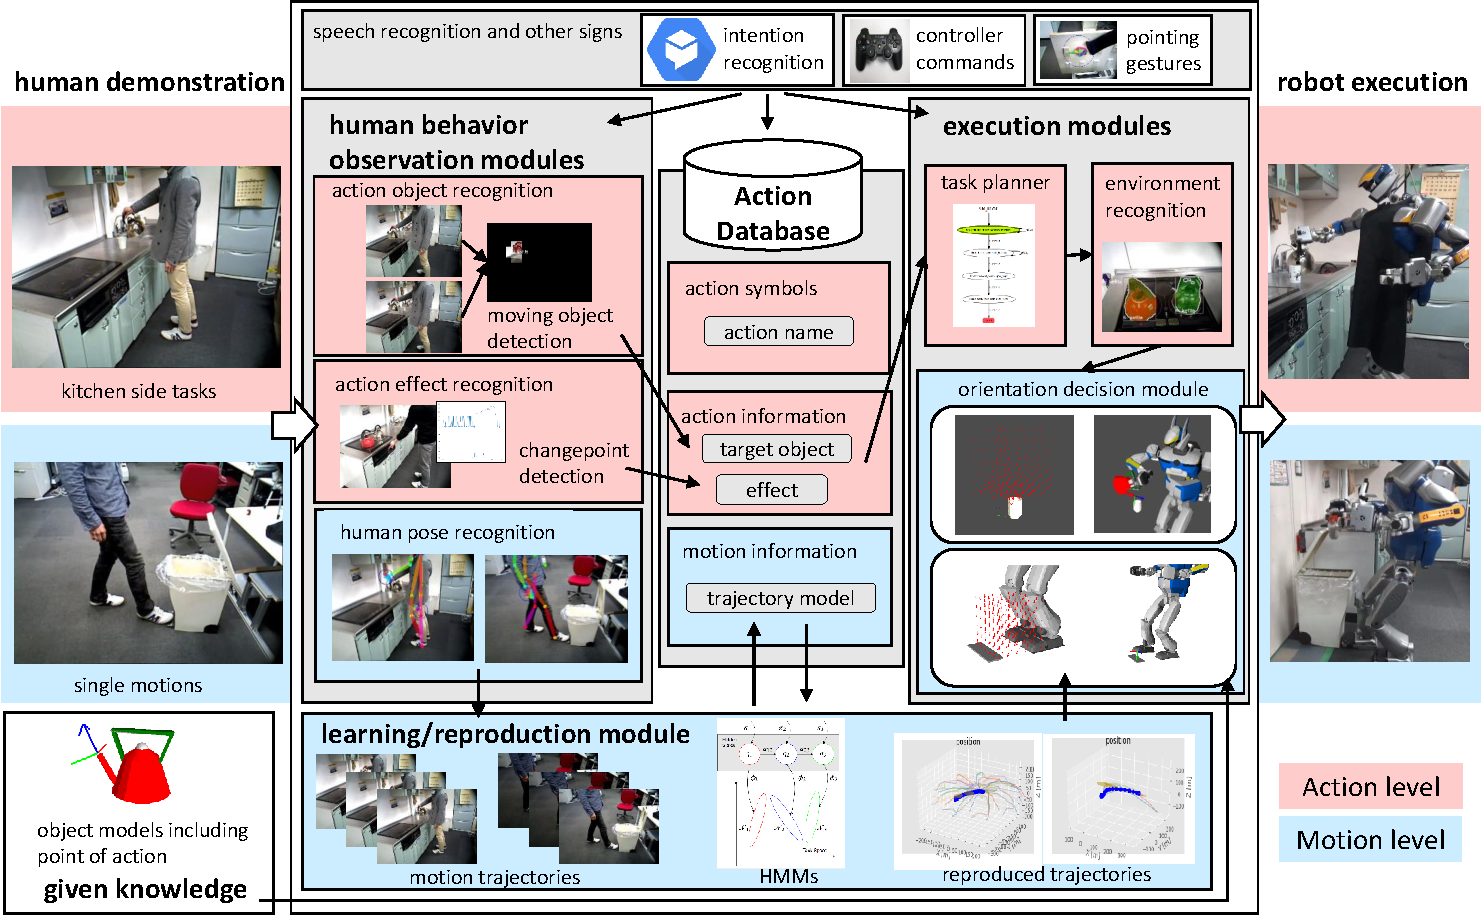
\includegraphics[width=1.0\columnwidth]{figs/system_approach_new}
    \caption{提案する新規動作獲得および実行システム}
    \label{figure:approach}
  \end{center}
\end{figure}

\section{提案手法}

\subsection{人間の行動観察に基づいた新規動作の獲得と実行}
\subsubsection{人間の動作観察}
人間の動作観察では,主に環境に働きかける部位として手先足先の認識を行う.
そこから得られた三次元位置の時系列データを,人間のデモンストレーションデータとしての入力情報とする.
また,ロボットの動作実行時において,人間による対象物や対象範囲の指示をロボットが理解するため,指差し認識を行う.

%% \begin{figure}[htbp]
%%   \begin{center}
%%     \begin{minipage}[t]{0.24\hsize}
%%       \begin{center}
%%         \includegraphics[clip, width=1.0\columnwidth]{figs/nowprinting}
%%         \subcaption{手先認識 (OpenPose)}
%%         \label{figure:SSDHand}
%%       \end{center}
%%     \end{minipage}
%%     \begin{minipage}[t]{0.24\hsize}
%%       \begin{center}
%%         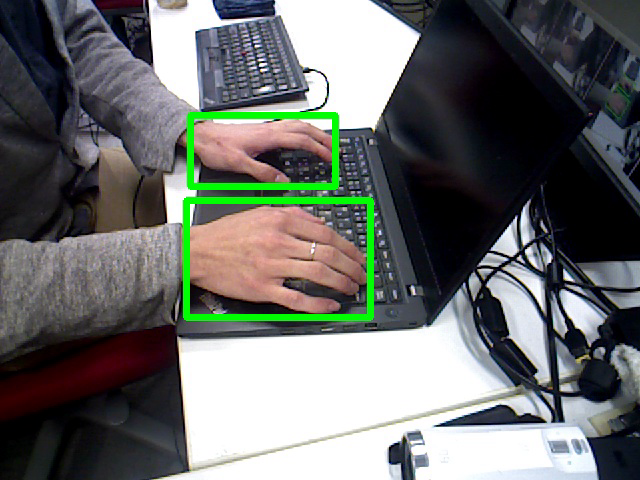
\includegraphics[clip, width=1.0\columnwidth]{figs/ssd_hand}
%%         \subcaption{手先認識 (SSD)}
%%         \label{figure:SSDHand}
%%       \end{center}
%%     \end{minipage}
%%     \begin{minipage}[t]{0.24\hsize}
%%       \begin{center}
%%         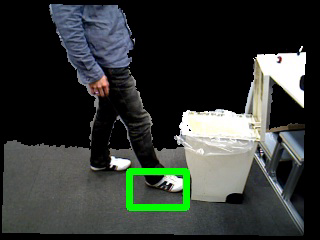
\includegraphics[clip, width=1.0\columnwidth]{figs/toe_bb}
%%         \subcaption{足先認識}
%%         \label{figure:OpenPoseFoot}
%%       \end{center}
%%     \end{minipage}
%%     \begin{minipage}[t]{0.24\hsize}
%%       \begin{center}
%%         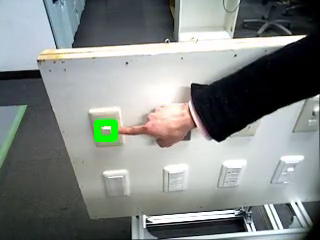
\includegraphics[clip, width=1.0\columnwidth]{figs/pointing}
%%         \subcaption{指差し認識}
%%         \label{figure:finger}
%%       \end{center}
%%     \end{minipage}
%%   \end{center}
%% \end{figure}

\subsubsection{確率モデルを用いた動作軌道の学習と再現}
本研究では,人間の手先認識や足先認識から得られた動作軌道をHidden Markov Model (HMM) を用いて学習する.入力を動作軌道の位置と速度を合わせたベクトル\(\vector{\zeta}_t = [\vector{x}_t, \dot{\vector{x}}_t]^\top\)の時系列データとし,EMアルゴリズムにより以下のパラメータを推定する.
\begin{itemize}
  \item 隠れ状態の出力確率\(\mathcal{N}_i(\vector{\mu}_i, \Sigma_i)\)
  \item 隠れ状態の遷移確率\(A\)
  \item 初期状態確率\(\Pi\)
\end{itemize}

学習されたHMMを用いた動作軌道の再現には,モデル予測制御 (MPC) の考え方を導入した手法を用いる.
\begin{align}
  \vzeta_{t+1} &= A \vzeta_{t} + B \vu_{t} \label{equation:linear} \\
  J &= (\vmu_s - \vzeta_s)^\top Q_s (\vmu_s - \vzeta_s) + \vu_s^\top R_s \vu_s \label{equation:mpc_cost}
\end{align}

動作軌道が\equref{linear}に示す線形系により表されるという前提のもとで,\equref{mpc_cost}に示すコスト関数を最小化するような入力\(\vu_s\)を求め,そのときの\(\vzeta_s\)を動作の再現軌道として導出する.そのとき,\equref{mpc_cost}中の\(\vmu_s\)および\(Q_s\)は,推定されたHMMのパラメータを用いて予測される隠れ状態系列\(s\)とそれぞれの隠れ状態に対応した出力確率\(\mathcal{N}_i(\vector{\mu}_i, \Sigma_i)\)を用いて構成される.

\figref{learning_reproduction}に,入力となる軌道列からHMMのパラメータの推定を行い,それらを用いて軌道を再現する過程を例で示す.

\begin{figure}[htbp]
  \begin{center}
    \begin{minipage}[t]{0.30\hsize}
      \begin{center}
        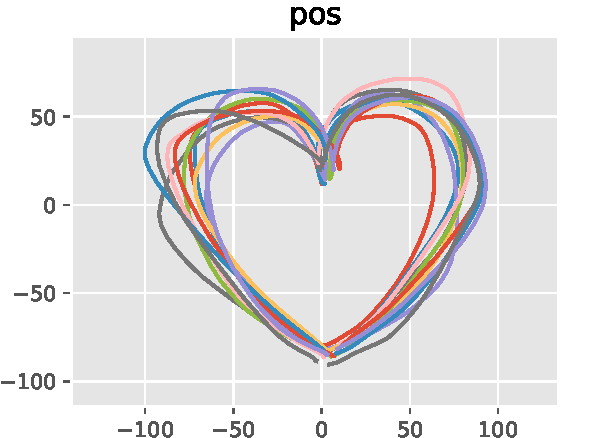
\includegraphics[clip, width=1.0\columnwidth]{figs/heart_orig_pos}
        \subcaption{入力軌道}
        \label{figure:input}
      \end{center}
    \end{minipage}
    \begin{minipage}[t]{0.30\hsize}
      \begin{center}
        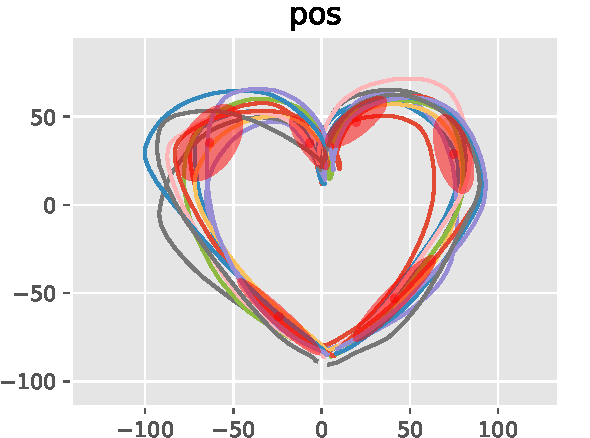
\includegraphics[clip, width=1.0\columnwidth]{figs/heart_hmm_pos}
        \subcaption{出力確率分布}
        \label{figure:HMM}
      \end{center}
    \end{minipage}
    \begin{minipage}[t]{0.37\hsize}
      \begin{center}
        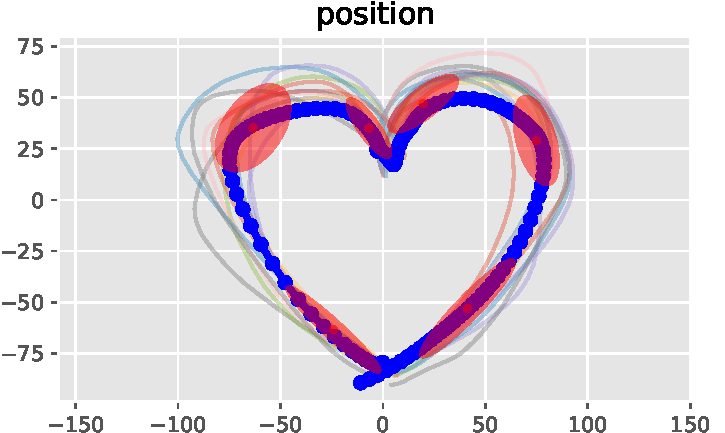
\includegraphics[clip, width=1.0\columnwidth]{figs/heart_mpc_pos}
        \subcaption{再現軌道}
        \label{figure:MPC}
      \end{center}
    \end{minipage}
    \caption{入力軌道に基づくHMMの学習により得られた出力確率分布とそれを用いた軌道の再現の例}
    \label{figure:learning_reproduction}
  \end{center}
\end{figure}

\subsubsection{ポテンシャル場による環境物体を考慮した動作の実行}
ロボットの動作決定のためには,目標位置と目標姿勢を決定する必要がある.
目標位置の時系列である動作軌道は前項の過程により得られる.
目標姿勢に関して本研究では,ポテンシャル場の考え方を導入し,環境操作物体を考慮した決定手法を提案する.
目標物体に対し手先を近づけるとき,一般的にその手のひらを物体の存在する方向に向けて近づけていく.
そのアイデアに着想を得て,目標環境物体の幾何モデルに対して,その物体の各面について,その面に「吸い付く」方向のベクトル場を空間に対して考え,その方向に手のひら (に代表される操作部位) を向けることによってその姿勢を与える.
電場に関するクーロンの法則を踏まえ,空間の各点\(\vector{r}\)における「物体に吸い付く力」を表すベクトル\(\vector{E}(\vector{r})\)を以下のように与える.

\begin{equation}
  \label{equation:electronic_potential_simple}
  \vector{E}(\vector{r}) = - \sum_{A' \in A} {\sum_{\vector{p} \in MG(A')} { \frac {\sigma'} {\| \vector{r} - \vector{r'}(\vector{p}) \| ^ 2} \cdot \frac {\vector{r} - \vector{r'}(\vector{p})} {\| \vector{r} - \vector{r'}(\vector{p}) \|} } }
\end{equation}

ここで,\(A\)は与えられた幾何モデルにおける面の集合,\(MG(A')\)は面\(A'\)内の格子点の集合を表す.
%% \equref{electronic_potential_simple}により,生成されたベクトル場の例を\figref{electronic_potential}に示す.
それぞれの矢印は,その矢印の始点の位置における物体に「吸い付く力」が働く方向を表す.
この向きに沿うような操作部位の姿勢を目標手先姿勢として与える.

%% \begin{figure}[htbp]
%%   \begin{center}
%%     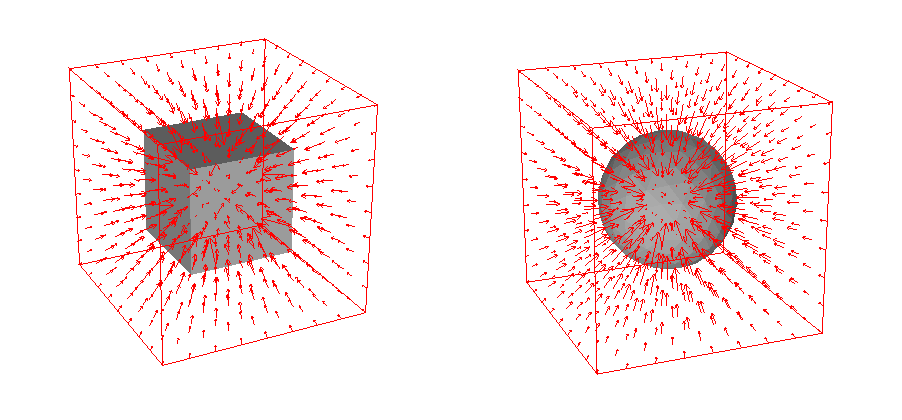
\includegraphics[width=0.70\columnwidth]{figs/electronic-potential-cube-sphere.png}
%%     \caption{三次元空間におけるポテンシャル場の様子.
%%       左図は立方体,右図は球体の例.
%%       小さな赤い矢印はそれぞれその始点の位置でのポテンシャル場の向きを表す.}
%%     \label{figure:electronic_potential}
%%   \end{center}
%% \end{figure}

\subsubsection{HRP-2を用いた動作実験}
ヒューマノイドHRP-2を用いて,人間のデモンストレーションをもとに獲得された動作の実行を行った.そのスナップショットを\figref{experiments}に示す.

\begin{figure}[htbp]
  \begin{center}
    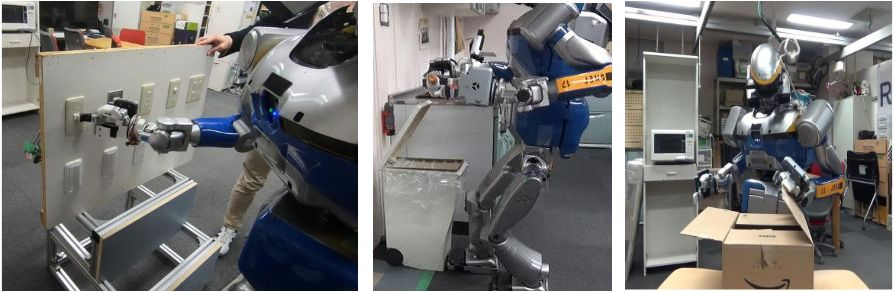
\includegraphics[width=1.0\columnwidth]{figs/experiments}
    \caption{ボタン押し,脚を用いたゴミ箱の蓋開け,箱の蓋閉め}
    \label{figure:experiments}
  \end{center}
\end{figure}

\subsection{人間の指示による動作の実行}
\subsubsection{人間によるタスク範囲の指示}
タスクによっては,雑巾がけのように,その目的に応じて操作範囲が変化する動作が考えられる.
そのような動作において,人間はロボットにそのタスク範囲を指示し動作の適切な実行を依頼できる必要がある.
そのために本研究では,%% \figref{pointing_area}に示すような,
指差しを用いて人間が動作のタスク範囲を指示できる枠組みを用意する.
ロボットはその指示された範囲に応じて動作軌道を拡大させることにより,タスクを達成することができる.

\begin{figure}[htbp]
  \begin{center}
    \begin{minipage}{0.48\hsize}
      \begin{center}
        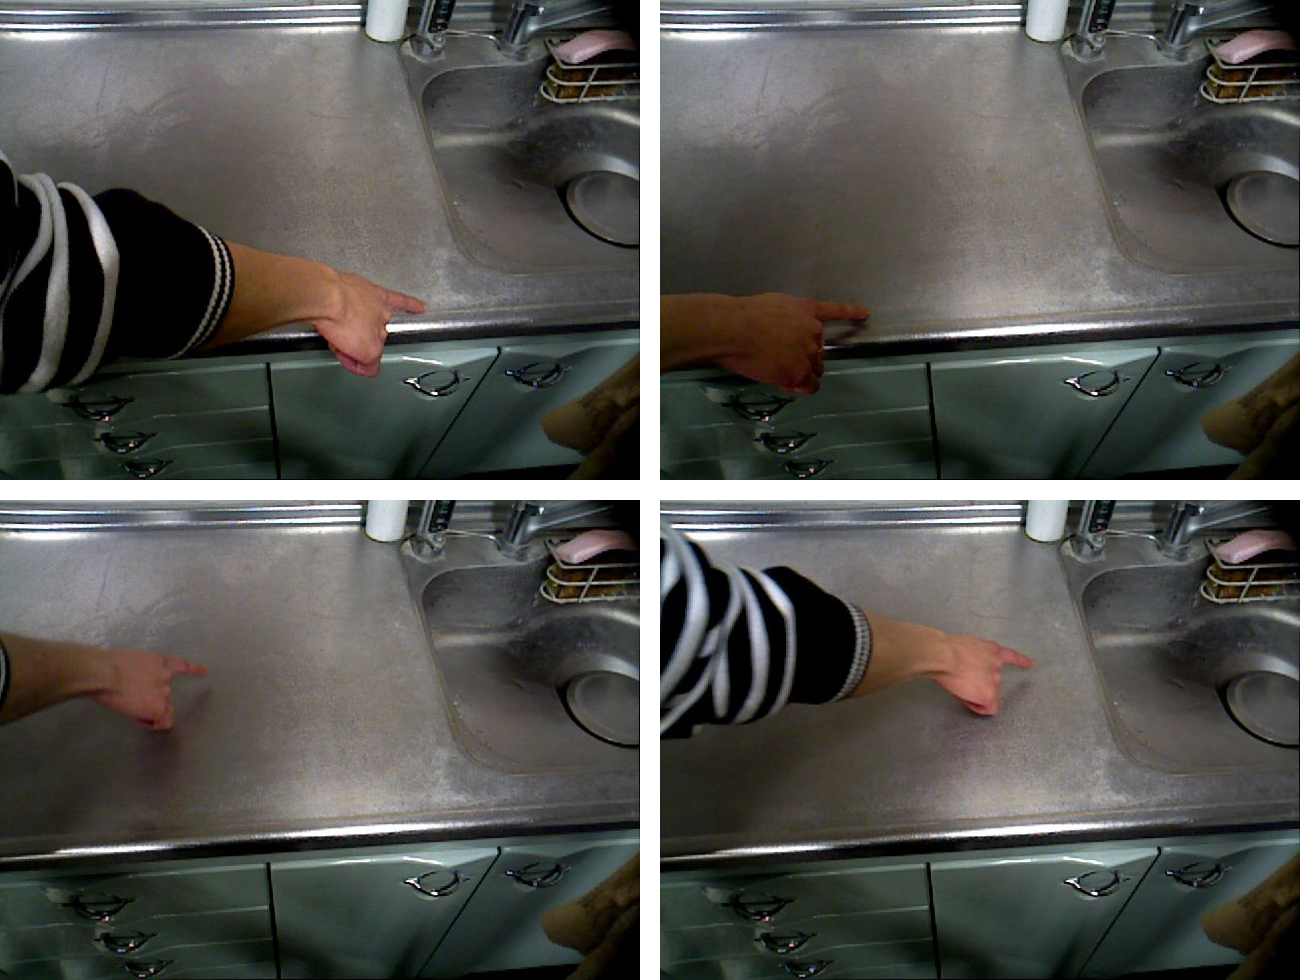
\includegraphics[clip, width=1.0\columnwidth]{figs/pointing_area_image}
      \end{center}
    \end{minipage}
    \begin{minipage}{0.48\hsize}
      \begin{center}
        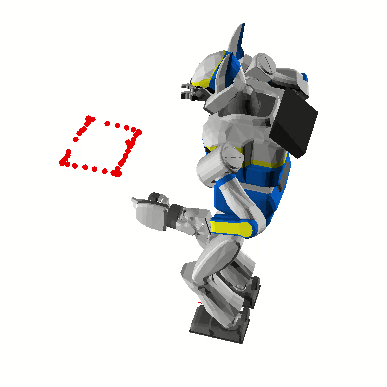
\includegraphics[clip, width=0.8\columnwidth]{figs/pointing_area}
      \end{center}
    \end{minipage}
    \caption{指差しにより範囲を指示する様子}
    \label{figure:pointing_area}
  \end{center}
\end{figure}

\begin{figure}[htbp]
 \begin{center}
  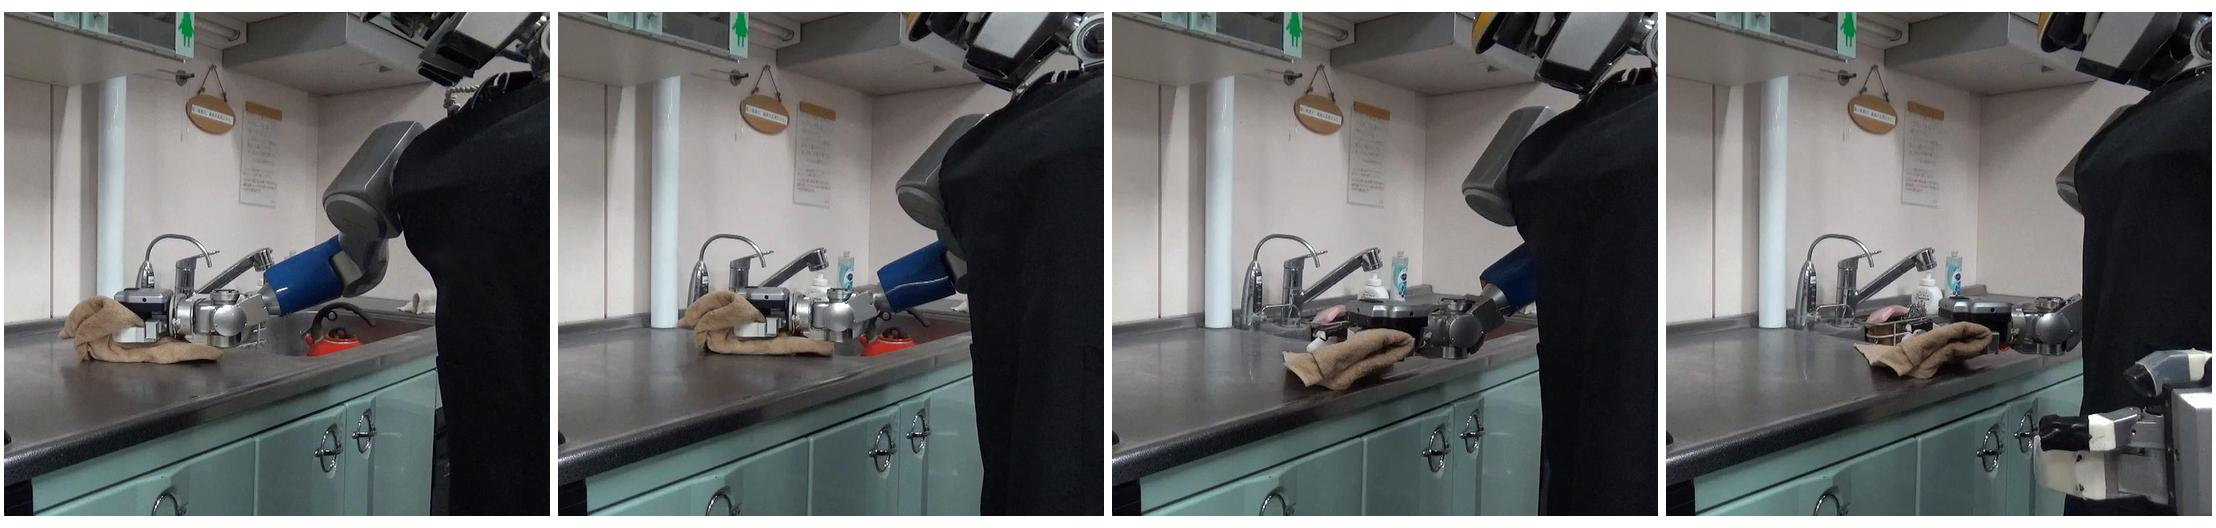
\includegraphics[width=1.0\columnwidth]{figs/wipe.jpg}
  \caption{人間の指示した範囲に対して雑巾をかける様子.}
  \label{figure:wipe}
 \end{center}
\end{figure}

\subsubsection{ジェスチャ演示による動作の連想呼び出し}
ロボットにやってほしい動作を人間が依頼する場合,目的となる動作に対してその動作名が紐付いていれば,その紐付けられた動作名を用いて特定の動作を指定できる.
一方で,そのように動作軌道と動作名が紐付けられていない場合,言葉によって動作を指定することができない.
そのような場合においてロボットに特定の動作を連想させ実行させる方法として,本研究では「ジェスチャ演示」を提案する.
動作名により紐付いていなくても,ロボットは既知動作に対する動作軌道を示す確率モデル情報を保有している.
それを応用して,人間がジェスチャで目的の動作を一度やってみせ,その演示動作軌道をロボットが持っている動作モデル群と比較することにより,どの動作を指し示しているかを判断する.
本研究ではその比較の対象として,演示軌道に対する各学習済みモデルを用いた際の生成コストを用いる.
コストはHMMのフォワーディングアルゴリズムを用いて算出され,すべての学習済みモデルに対する算出コストが最も小さかった動作を目的とする動作であるとして,ロボットはその動作の実行を試みる.

\section{結論}
本研究では,人間の行動観察に基づいた,ロボットの新規動作の獲得およびその新規獲得動作の人間の指示や依頼に応じた実行を目的とし,それを実現するシステムを提案した.
新規動作獲得においては,人間のデモンストレーションにおける動作軌道を確率モデルを用いて学習および再現し,また,環境物体のポテンシャル場という考え方を導入し,実環境のロボットの動作を決定した.
また,人間の指示に応じた実行として,人間が指示するタスク範囲やジェスチャ演示に応じて,動作の修正または選択を行える枠組みを備え,タスクに応じた動作の実行を可能にした.

\bibliographystyle{junsrt}
\bibliography{p-report}

\end{document}

